\documentclass{article}

\usepackage[margin=1in]{geometry}
\usepackage[dvipsnames]{xcolor}
\usepackage{graphicx}
\usepackage{wrapfig}
\usepackage{setspace}
\usepackage{tabularx}
\newcolumntype{b}{>{\hsize=2\hsize\raggedleft\arraybackslash}X}
\newcolumntype{m}{>{\hsize=0.9\hsize\centering\arraybackslash}X}
\newcolumntype{s}{>{\hsize=0.7\hsize\centering\arraybackslash}X}
\usepackage{fancyhdr}
\pagestyle{fancy}
\fancyhf{}
\renewcommand{\headrulewidth}{0pt}
\fancyfoot[C]{\textcolor{white}{\thepage}}
\definecolor{BgColour}{HTML}{2f3c63}
\pagecolor{BgColour}
\color{white}
\onehalfspacing

\usepackage[sfdefault]{noto}
\newfontfamily\DejaSans{DejaVu Sans}

\begin{document}

\begin{wrapfigure}{l}{0.3\textwidth}
    \vspace*{-1cm}
    \centering
    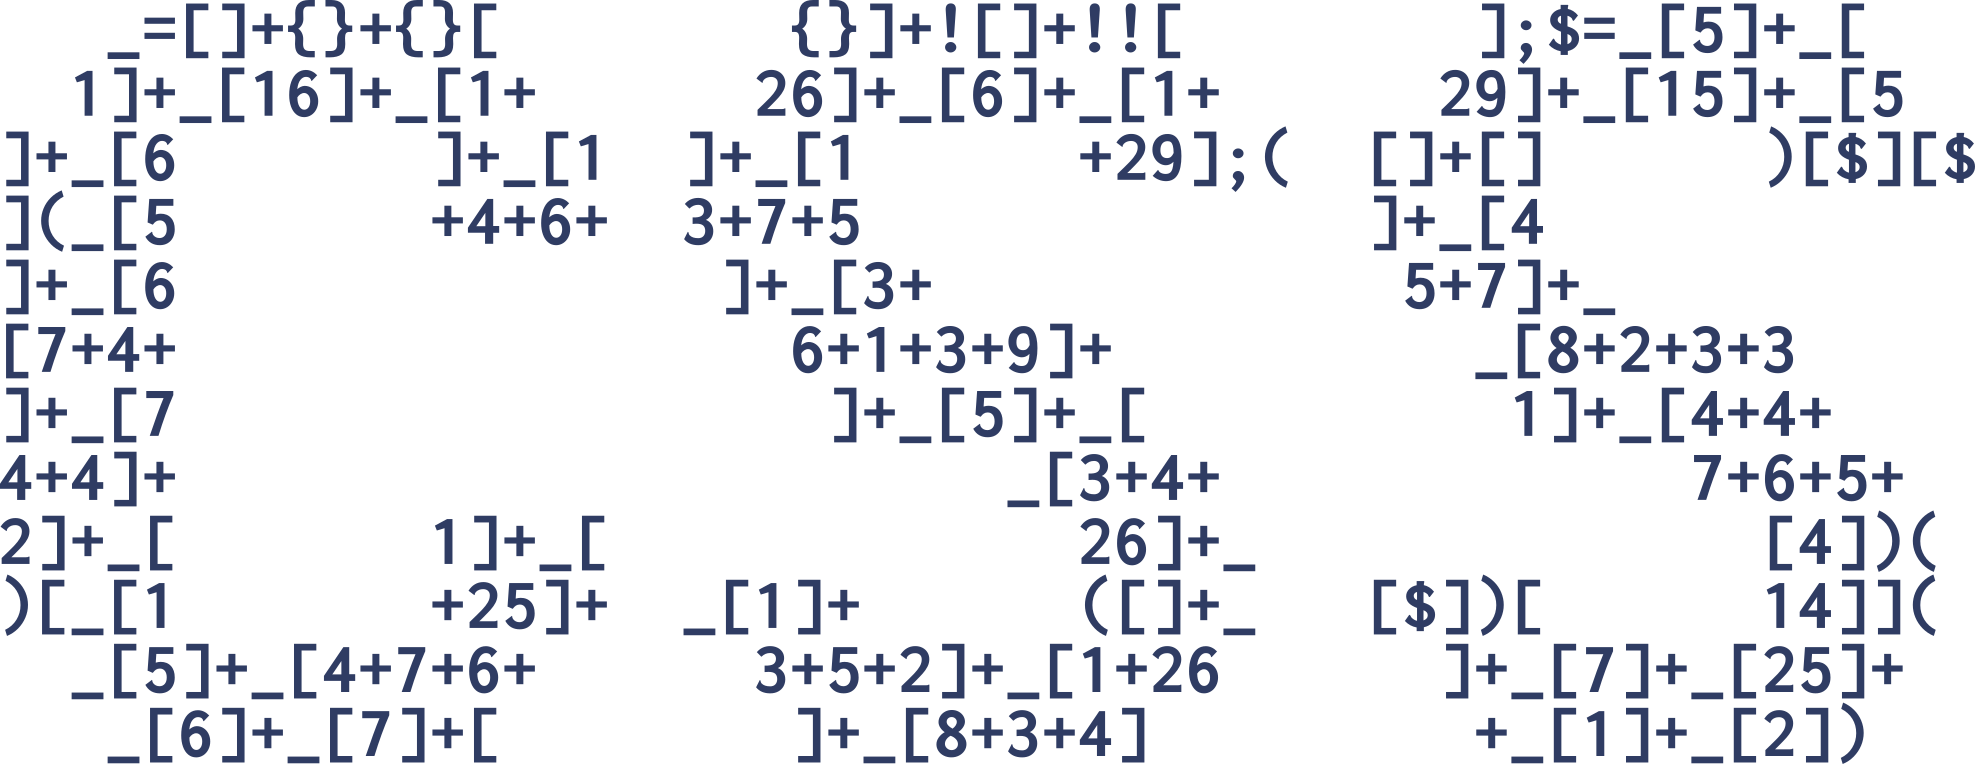
\includegraphics[width=0.3\textwidth]{CSS_Logo}
\end{wrapfigure}

\vspace*{1cm}

\Huge

\noindent \hspace{0.5cm}\textbf{Sponsorship Proposal}

\par

\noindent \hspace{0.5cm}\textbf{2019/20}

\vspace{1.5cm}

\fontsize{11}{14}\selectfont

Computer Science Society (CSS) is the departmental society for Computer
Science at the University of Birmingham. With over 180 members and a
range of initiatives, we work closely with the School of Computer
Science, our sponsors and the local and wider tech communities to
provide our members with experience and skills that will be invaluable
to them in their careers.\medskip

\noindent Some of the events and initiatives we run (or help to run) for our
members are:\medskip

\begin{itemize}
\item
  \textbf{HackTheMidlands}, a 24-hour hackathon open not only to
  students but to anyone interested (aged 14+) with around 150 attendees
  last time.
\item
  \textbf{The Women in Technology Conference}, hosted alongside WISE
  (Women in Science and Engineering) and oSTEM (Out in Science,
  Technology, Engineering and Maths) - a day-long conference focussed on
  empowering and equipping women in technology, to provide confidence
  and combat the gender imbalance in the field.
\item
  \textbf{CSS Hardware Lab} - State of the art technology that we use to
  provide our members with hands-on experience of bleeding-edge
  technology such as Virtual Reality. Not only do we use the Hardware
  Lab for our members, we also use it to give back to the tech community
  by providing in-kind sponsorship for events such as hackathons, to
  enrich the experiences of attendees across the country.\medskip
\end{itemize}

As well as these, we run a variety of social and tech events across the
academic year, including (but not limited to), seminars, talks,
workshops, hackathon/conference trips, LAN parties, games nights and
much more.\medskip

We would love to work with you in the coming year to deliver
this, and none of this would be possible without you! So if you're
interested in working with us to provide skills, insight, experience and
confidence to our members (and more!), let us know! On the following
page are the sponsorship tiers that we are offering this year.

\newpage

\renewcommand{\arraystretch}{2}
\begin{tabularx}{\textwidth}{ b  s  s  s  m }
    & Bronze (£750) & Silver (£1500) & Gold (£2500) & Exclusive Partner\linebreak(£Negotiable) \\
    Logo on all society promotional material & {\DejaSans ✔} & {\DejaSans ✔}& {\DejaSans ✔}& {\DejaSans ✔}\\
    Mail shot(s) (Monthly Digest) per month & 0 & 1 & 2 & 3 \\
    Mail shot(s) (immediate) per month & 0 & 0 & 1 & 2 \\
    Society-wide promotion of company schemes \& initiatives (eg. internships, placements) & & {\DejaSans ✔}& {\DejaSans ✔}& {\DejaSans ✔}\\
    Company-hosted events across the year & & {\DejaSans ✔}& {\DejaSans ✔}& {\DejaSans ✔}\\
    Right of first-refusal to the sponsorship tier the following year & & & & {\DejaSans ✔}\\
    Ability to display company banner alongside society banner (eg. in School of Computer Science) & & & {\DejaSans ✔}& {\DejaSans ✔}\\
    Distribution of promotional material & & & {\DejaSans ✔}& {\DejaSans ✔}\\
    Further negotiable benefits & & & & {\DejaSans ✔}\\
\end{tabularx}

\vspace{1cm}

NB: All sponsorship packages are negotiable within reason.

\end{document}
